% !TEX root = main.tex
\begin{figure}[t]
\begin{center}
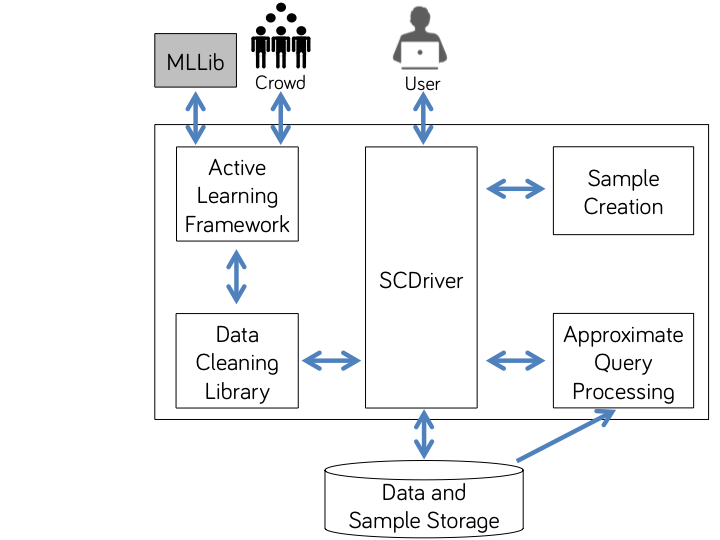
\includegraphics[width=3.5in]{figures/system-architecture}
\end{center}
\caption{The \system{} system architecture.}
\label{f:system-architecture}
\end{figure}

\section{System Overview}
Figure~\ref{f:system-architecture} shows the high-level system architecture of \system. ...describe the diagram... mention that data cleaning library is easy for data cleaning experts to extend, a la mllib., etc.

\subsection{Data Cleaning for Query Answering}
Ways to clean data:
\begin{itemize}
\item Use the crowd to clean data (slow, costly, high quality)
\item Use automated methods to clean data (fast, cheap, lower quality)
\end{itemize}

Ways to answer queries on dirty data:
\begin{itemize}
\item Clean a sample and use AQP to infer the query result.
\item Clean a sample, use it to train a model, use the model to clean a larger sample, and use AQP to infer the query result.
\item Clean a sample, use it to train a model, use the model to clean the rest of the data, answer the query.
\end{itemize}

We support all of these. 
Doing so is hard because using the crowd/training models/automated cleaning all have very different timescales.

\subsection{Progressive Data Cleaning}
\begin{itemize}
\item To resolve the above problem, we do \textit{progressive data cleaning}. 
\item That is, data cleaning occurs asynchronously during analytics, and each successive analytics task operates on increasingly clean data. 
\item This allows pay-as-you-go cleaning (only clean data relevant to your workload, stop cleaning whenever you want).
\item It's especially valuable when subsequent operations/queries in your application reuse data you began cleaning during earlier steps (e.g., drill-down exploratory analytics, real-time dashboards that refresh).
\item This work-sharing of cleaned data generalizes to settings where many concurrent users analyze the same data. Supporting such a workflow is future work.
\end{itemize}

\subsection{Cleaning with Crowds}
\begin{itemize}
\item Automated methods only get you so far
\item Crowds are often good at tasks where automated methods fail (e.g. deduplication, sentiment analysis, etc.)
\item But they're slow.
\item Our system makes using crowds for data cleaning on big analytics data practical in 3 ways:
	\begin{enumerate}
	\item We use sampling + AQP to limit the number of things the crowd has to clean
	\item We use active learning to limit the number of things the crowd has to clean (and intelligently select the things to clean)
	\item We use asynchrony to keep the crowd's latency from affecting query latency.
	\end{enumerate}
\item Still, there are serious challenges here to making the crowd affordable, high-quality, faster, and generalizable.
\end{itemize}

\subsection{Composing Data Cleaning Operations}
\begin{itemize}
\item Data is probably dirty in more than just one way. You shouldn't be limited to one cleaning task per query workload.
\item Challenge: how do you compose these operations? Which ones can run in parallel? How do you tell if cleaning operators won't touch the same data?
\item We provide a declarative framework for pipeline specification that allows operations to be either synchronous or asynchronous
\item Optimizing/reordering this pipeline remains future work.
\end{itemize}

\subsection{Beyond Query Answering}
\begin{itemize}
\item Many of our techniques are more general than just aggregate query answering.
\item There are other data analysis tasks that could benefit from progressive data cleaning.
\item E.g. feature engineering / model testing on dirty data.
\end{itemize}
